\documentclass[a4paper]{report}
\setlength{\headheight}{12.0pt}
\usepackage[T2A]{fontenc}
\usepackage[utf8]{inputenc}
\usepackage[russian,english]{babel}
\usepackage[left=25mm, top=20mm, right=25mm, bottom=30mm, nohead, nofoot]{geometry}
\usepackage{amsmath,amsfonts,amssymb} % математический пакет
\usepackage{fancybox,fancyhdr}
\usepackage{xcolor}
\usepackage{hyperref}
\usepackage{tkz-euclide}
\usepackage{enumitem}
\usepackage{amsmath}
\usepackage{pgfplots}
\usepackage{float}
\usepackage{fvextra}
\usepackage[cache=false]{minted}
\usepackage[figurename=Изображение]{caption}
\captionsetup[table]{name=Таблица}
\usemintedstyle{vs}

\hypersetup{colorlinks=true, allcolors=[RGB]{010 090 200}} % цвет ссылок
\newcommand{\lr}[1]{\left({#1}\right)} % команда для скобок
\pagestyle{fancy}
\fancyhf{}
\renewcommand{\headrulewidth}{0pt}
\fancyfoot[R]{\thepage}
\fancypagestyle{plain}{
    \fancyhf{}
    \fancyfoot[R]{\thepage}
    \renewcommand{\headrulewidth}{0pt}
}
\setcounter{page}{1} % счетчик нумерации страниц
\headsep=10mm
\definecolor{green_india}{HTML}{138808} % INDIA GREEN
\definecolor{green_light}{HTML}{90EE90} % LIGHT GREEN
\definecolor{green_slimy}{HTML}{299617} % SLIMY GREEN
\makeatletter
\def\@seccntformat#1{\csname #1ignore\expandafter\endcsname\csname the#1\endcsname\quad}
\let\latex@numberline\numberline
\def\numberline#1{\if\relax#1\relax\else\latex@numberline{#1}\fi}
\makeatother
\renewcommand{\thesection}{\arabic{section}.}
\renewcommand{\thesubsection}{\arabic{subsection}.}

\begin{document}
\subsection{Диаграмма пакетов}
\begin{figure}[H]
    \centering
    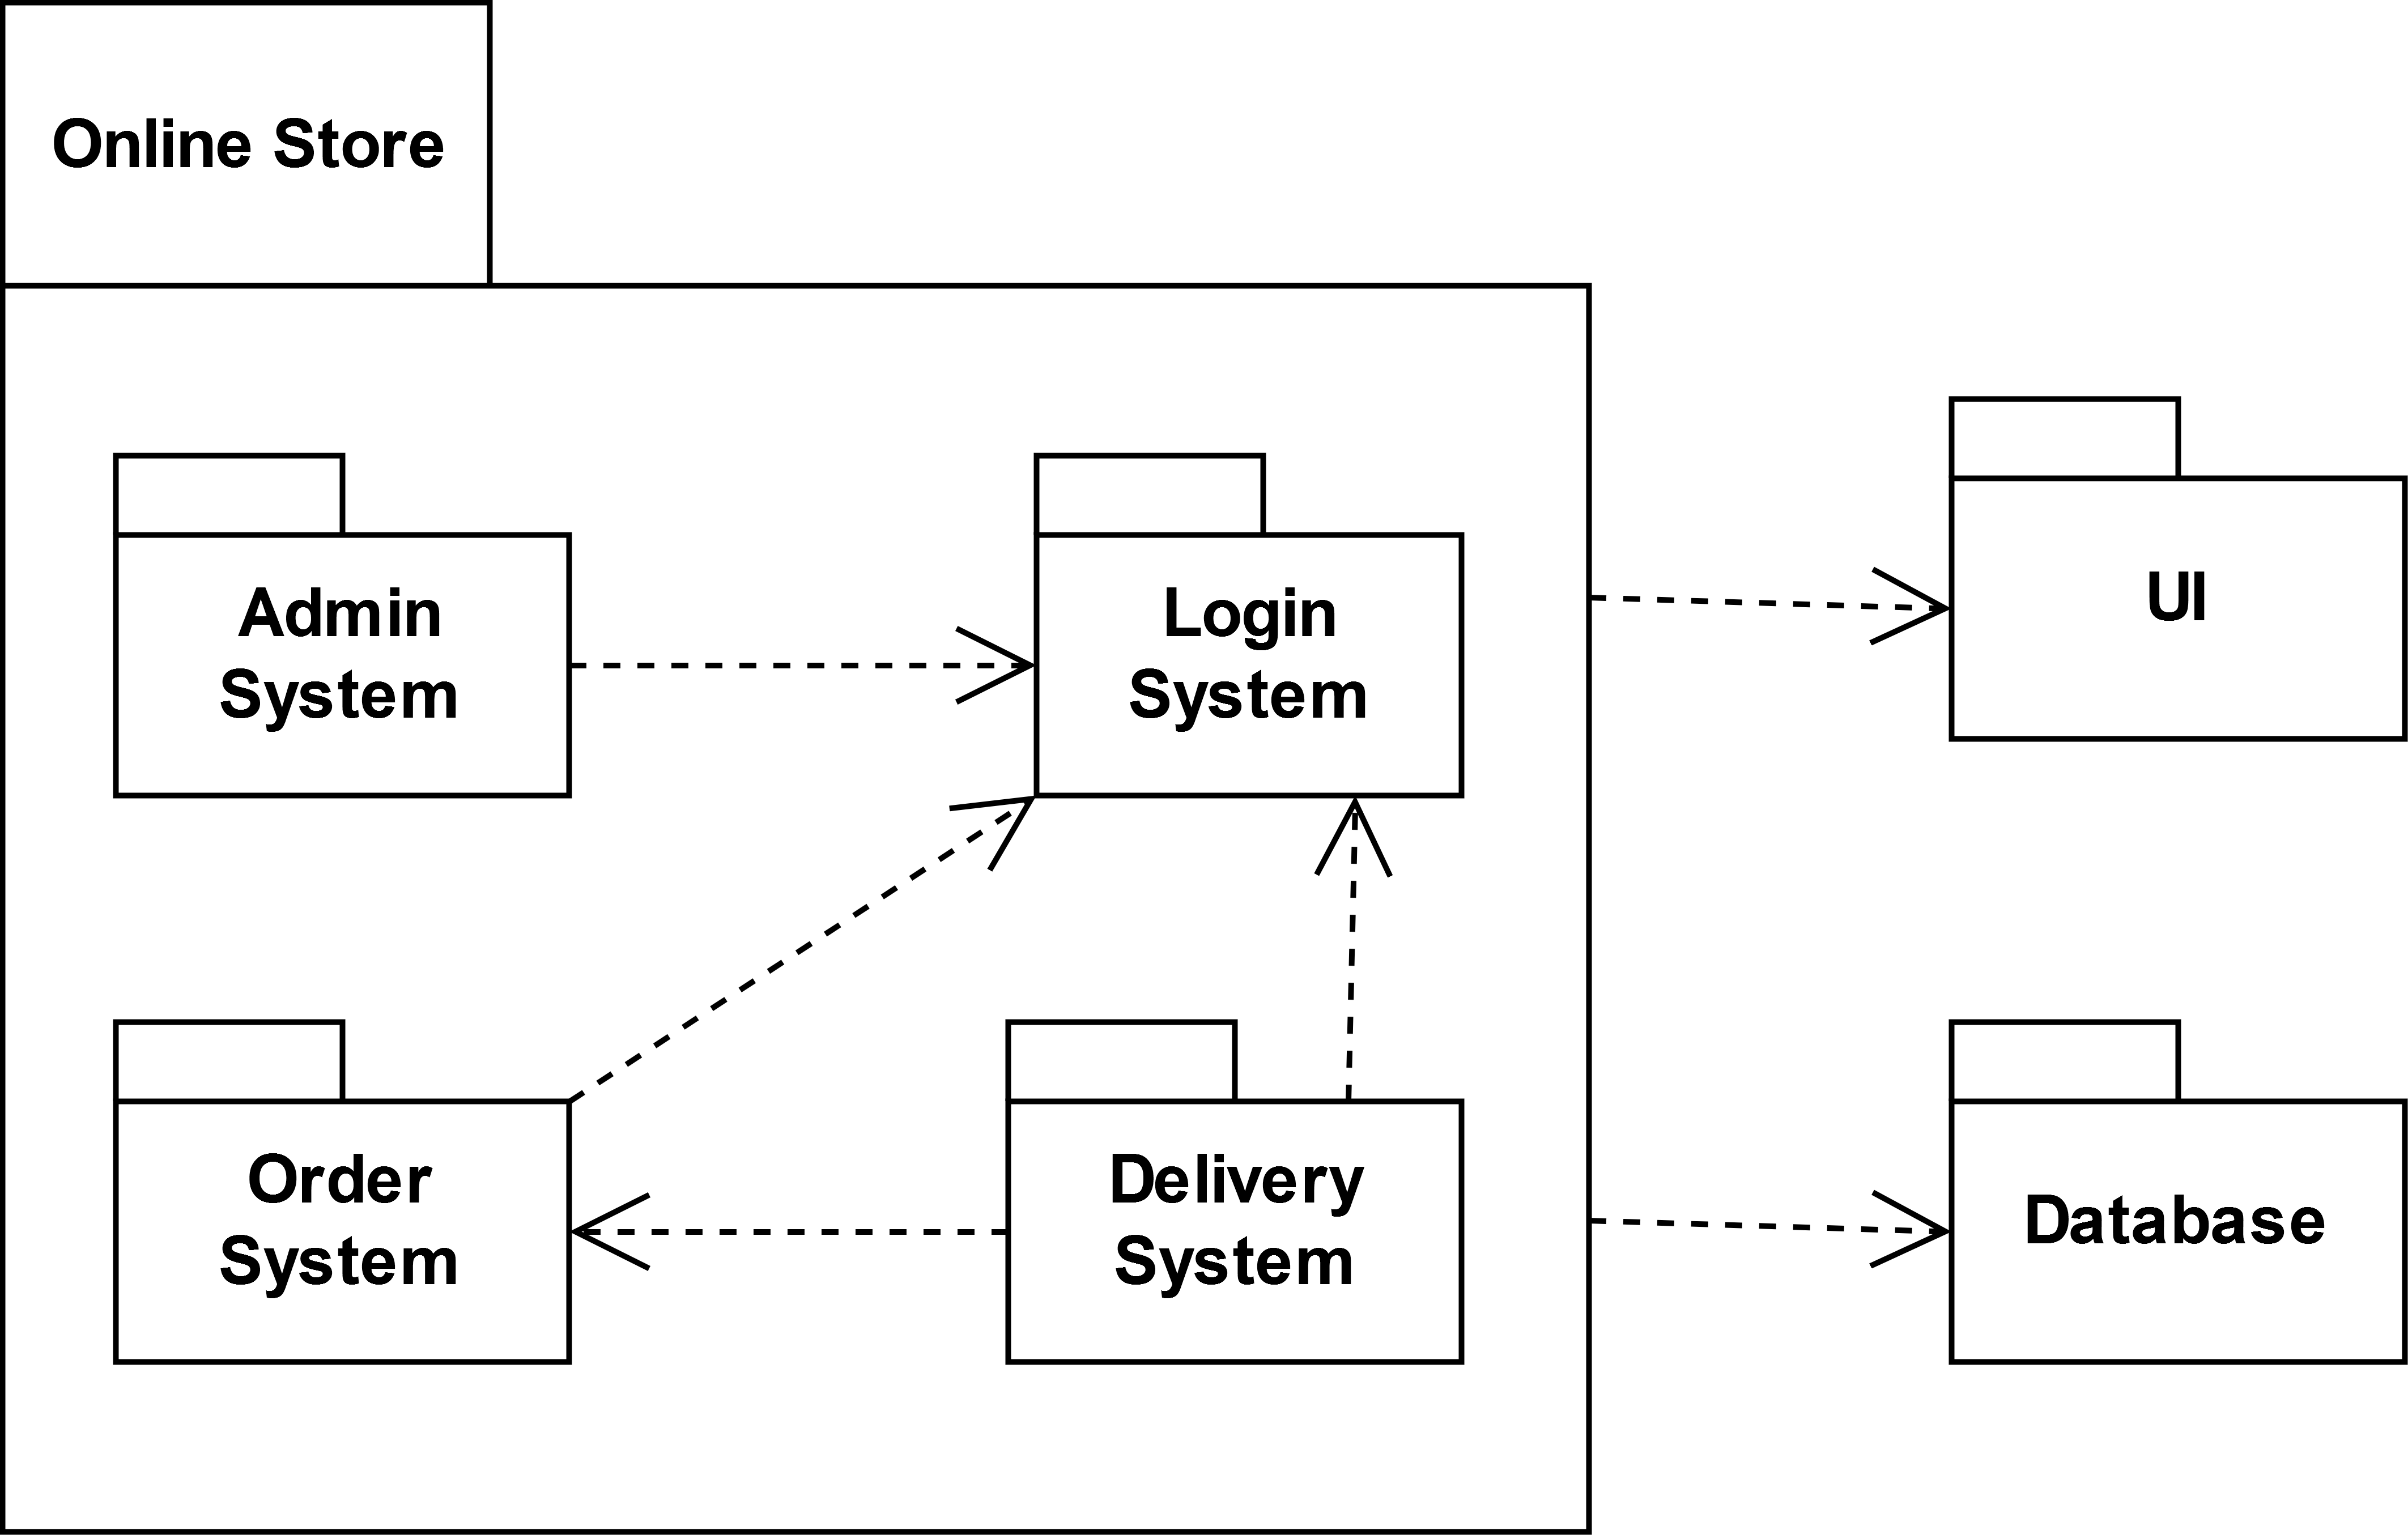
\includegraphics[width=0.6\textwidth]{Диаграмма пакетов.png}
\end{figure}
Описание:
\begin{enumerate}
    \item \textbf{Admin System:} Управляет административными функциями;
    \item \textbf{Order System:} Отвечает за обработку заказов, включая их создание, обновление и хранение;
    \item \textbf{Database:} Центральное хранилище данных, используемое всеми системами;
    \item \textbf{Online Store:} Компонент, предоставляющий функционал интернет-магазина, включая витрину товаров и работу с заказами;
    \item \textbf{Delivery System:} Система, обеспечивающая управление доставкой товаров;
    \item \textbf{Login System:} Отвечает за аутентификацию и авторизацию персонала;
    \item \textbf{UI (User Interface):} Пользовательский интерфейс для взаимодействия с системой;
    \item \textbf{Web:} Связывает пользовательский интерфейс с системой через интернет, используя соответствующую инфраструктуру.
\end{enumerate}
На диаграмме показаны составляющие элементы пакета \textbf{Online Store}: пакеты \textbf{Admin System, Login System, Order System} и \textbf{Delivery System. Admin System} взаимодействует с \textbf{Login System} для \textit{CRUD} пользователей, \textbf{Order System} и \textbf{Delivery System} взаимодействуют с \textbf{Login System} для получения информации о пользователе, \textbf{Delivery System} взаимодействует с \textbf{Order System} для получения информации о заказе. Главная по функциональности часть \textbf{Online Store} взаимодействует с пакетом графического интерфейса \textit{UI} для \textit{веб-} и \textit{мобильной} вёрстки, а также с пакетом \textit{Database}, для хранения данных.
\subsection{Диаграмма компонентов}
\begin{figure}[H]
    \centering
    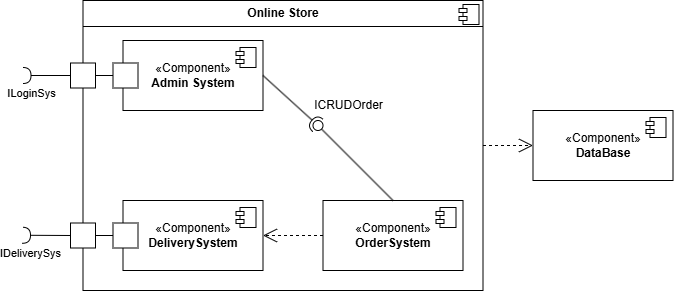
\includegraphics[width=\textwidth]{Диаграмма компонентов.png}
\end{figure}
Описание:
\begin{enumerate}
    \item \textbf{Online Store:} основной контейнер, в который входят все компоненты системы;
    \item \textbf{Admin System:} компонент, отвечающий за административные функции. \begin{enumerate}
        \item  Он требует интерфейс \textit{ILoginSys}, для аутентификации пользователей;
        \item Он требует интерфейс \textit{ICRUDOrder}, взаимодействуя с системой управления заказами \textbf{OrderSystem}.
    \end{enumerate}
    \item \textbf{Order System:} компонент, управляющий заказами. \begin{enumerate}
        \item Он предоставляет интерфейс \textit{ICRUDOrder}, предоставляет функционал для управления заказами;
        \item Он использует компонент \textbf{Delivery System}, для получения информации о заказах для их доставки..
    \end{enumerate}
    \item \textbf{Delivery System:} Отвечает за обработку и управление доставкой заказов. \begin{enumerate}
        \item Он требует интерфейс \textit{IDeliverySys}, для обмена данными о заказе;
        \item Он используется компонентом \textbf{Order System}, для получения информации о заказах для их доставки.
    \end{enumerate}
    \item \textbf{DataBase:} Компонент базы данных, отвечающий за хранение данных системы, для записи информации о новых заказах, хранении информации о пользователе, и о самих товарах (Все компоненты \textbf{Online Store} его используют).
\end{enumerate}
\subsection{Диаграмма развёртывания}
\begin{figure}[H]
    \centering
    \includegraphics[height=0.8\textheight]{Диаграмма развёртывания.png}
\end{figure}
Описание:
\begin{enumerate}
    \item \textbf{Рабочая станция пользователя (User Workstation)}\\
    На стороне клиента используется:
    \begin{itemize}
        \item \textbf{Web Browser} -- среда выполнения, предназначенная для работы с интерфейсом приложения. Веб-браузер выполняет React-приложение, которое загружается с веб-сервера.
    \end{itemize}
    
    \item \textbf{Веб-сервер (Web Server)}\\
    Веб-сервер отвечает за предоставление фронтенда клиенту. Его компоненты:
    \begin{itemize}
        \item \textbf{Frontend (React)} -- артефакт, представляющий собой React-приложение, которое используется для пользовательского интерфейса.
        \item \textbf{Node.js} -- среда выполнения для сборки и (при необходимости) серверного рендеринга React.
    \end{itemize}
    
    \item \textbf{Сервер приложений (Application Server)}\\
    Сервер приложений обрабатывает бизнес-логику и взаимодействует с базой данных. Компоненты сервера приложений:
    \begin{itemize}
        \item \textbf{Backend (Django/Express.js)} -- артефакт, представляющий серверную часть веб-приложения.
        \item \textbf{Python Interpreter} -- среда выполнения, если сервер написан на Django.
        \item \textbf{Node.js Runtime} -- среда выполнения, если серверная часть реализована на Express.js.
    \end{itemize}
    
    \item \textbf{Сервер базы данных (Database Server)}\\
    Сервер базы данных хранит всю информацию о продуктах, пользователях и заказах. Используется:
    \begin{itemize}
        \item \textbf{SQLite Database} -- встроенная база данных, не требующая отдельной среды выполнения.
    \end{itemize}
    
    \item[*]\textbf{Взаимодействие между компонентами}\\
    \begin{enumerate}
        \item Пользователь через Web Browser отправляет HTTP-запрос на Web Server.
        \item Web Server передаёт запрос на Application Server для обработки бизнес-логики.
        \item Application Server отправляет SQL-запросы к SQLite Database для получения или обновления данных.
        \item Ответ от базы данных возвращается на Application Server, а затем обратно на Web Server.
        \item Web Server формирует и отправляет HTTP-ответ пользователю.
    \end{enumerate}
\end{enumerate} 

\end{document}